\documentclass[../../Problems]{subfiles}
\begin{document}
\subsection{Peace}{\label{pp:peace}}
\textbf{Problem Statement:}\\
Draw the outline of the Proportionl Peace Sign according to measurements as shown in \ref{fig:peacemeasurements}.
\begin{figure}[H]
\centering
	\begin{subfigure}{\linewidth}
	\centering
	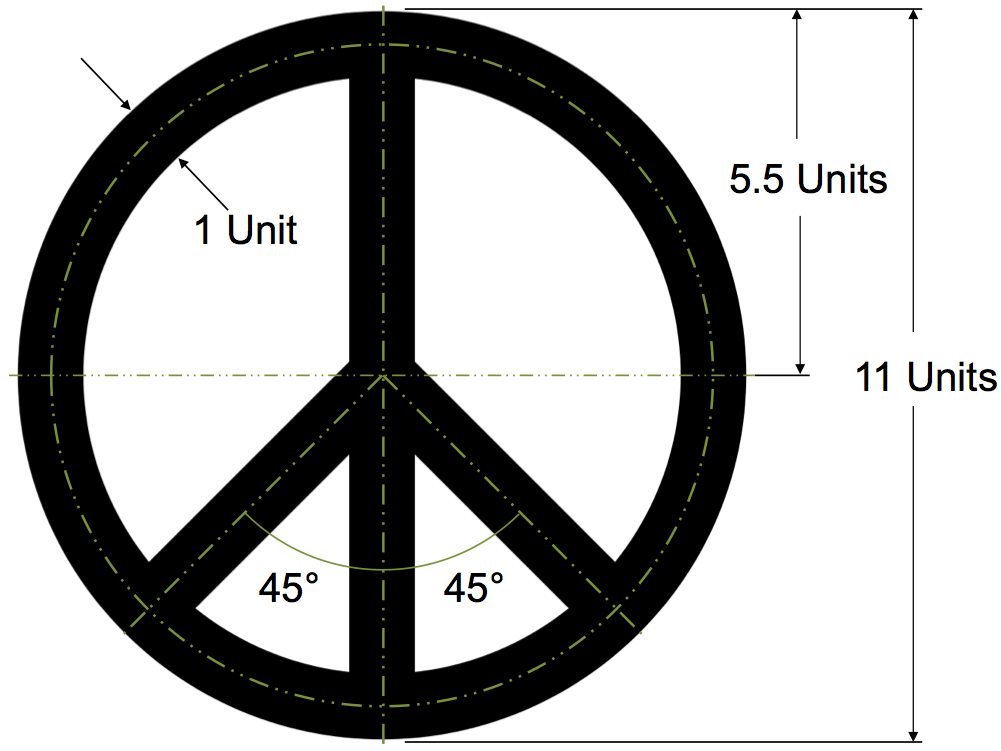
\includegraphics[height = 0.4\linewidth]{Peace Measurements.png}
	\caption{\href{https://bit.ly/peace-sign-measurements}{Measurements} by Jerry S. Sadin, based on (\href{https://bit.ly/peace-sign-wikipedia}{image} by \href{https://commons.wikimedia.org/wiki/User:SchuminWeb}{SchuminWeb})}
	\label{fig:peacemeasurements}
\end{subfigure}
\begin{subfigure}{\linewidth}
	\centering
	
\includegraphics[height = 0.4\linewidth]{Peace.png}
	\caption{Output generated using Simplecpp}
	\label{fig:peace}
\end{subfigure}
\caption{Peace Sign}
\end{figure}
The output image will look like \ref{fig:peace}.
\begin{funvideo}
\href{https://youtu.be/GO5FwsblpT8}{Carl Sagan's Pale Blue Dot -- carlsagandotcom}\\
\href{https://youtu.be/lshWT0iyxds}{Cosmos: Possible Worlds (Carl Sagan's Monologue) -- Evil Dead}
\end{funvideo}
\end{document}